\appendix

\section{Performance Collection Implementation Details}\label{appendix1}


In this work, we have developed the \textit{pipeline\_collector} suite, aimed at collecting detailed time-series information from distributed scientific pipelines. 

The \textit{tcollector} package is a python software suite that can collect system performance data at predetermined intervals. The package is designed to monitor the performance statistics for web-servers and cluster nodes. The tcollector software records time series of the different performance metrics and sends them to a Time Series Database through HTTP. The Time Series Database, OpenTSDB stores the data in an HBase \citep{hbase} instance at the performance collection server. Users interested in plotting time series can plot real time or historical data through an HTTP interface with OpenTSDB. With a central performance collection server, data from multiple processing sites can be collected and analyzed. 

Tcollector formats the time series information in four fields. First is the name of the metric which is measured. Second is the UNIX timestamp. Third is the time series recorded as an integer or a float. Finally, a set of tags (key-value pairs) can be added to the data point. These four fields are discussed below and can be seen on the right side of Figure \ref{fig:tsdb_tcollector}. 

\begin{figure}[!h]
    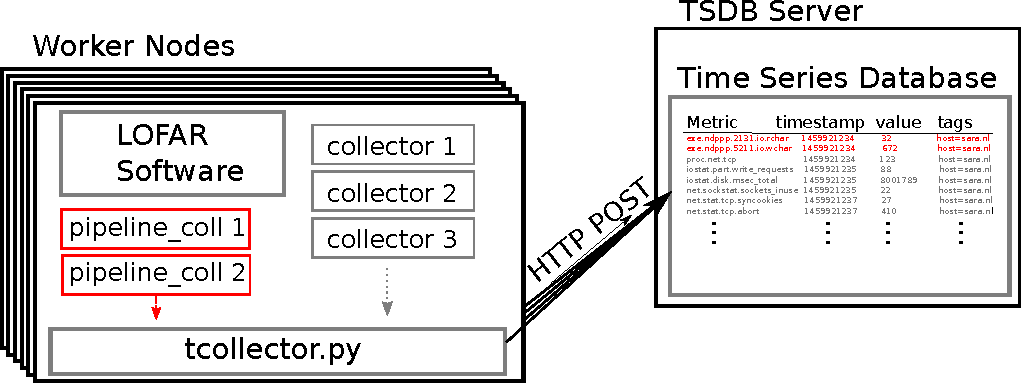
\includegraphics[width=\linewidth]{ch4/figures/figA14/TSDB_tcollector.pdf}
      \caption{Communication between worker nodes and the TSDB server, including the pipeline\_collector modules (in red). The \textit{pipeline\_collector} suite collects information on the running LOFAR pipelines, while the rest of the tcollector package collects system performance data. The existing tcollector package and its collectors are shown in gray. The collectors in gray only record metrics from the global system. }
	\label{fig:tsdb_tcollector}
\end{figure}

\subsection{The pipeline\_collector suite}\label{sec:customcollectors}



The tcollector package cannot collect data on individual processes, nor can it associate these processes with specific steps of a data processing pipeline. We've supplemented the software with the \textit{pipeline\_collector} suite\footnote{Located at https://gitlab.com/apmechev/procfs\_tcollector.git} using an executable that monitors a pipeline's running processes\footnote{Located at https://github.com/apmechev/procfsamp}. When an executable that is part of the LOFAR pipeline launches, a dedicated collector begins reporting information on the individual process. Every time a new processing step starts, the \textit{prefactor} pipeline records the step name in a log file. \textit{pipeline\_collector} determines the current running step using this log. Running the LOFAR processing concurrently with the tcollector package gives us per-step performance data without changing or slowing down the LOFAR \textit{prefactor} pipeline. Furthermore, \textit{pipelie\_collector} can be integrated with any processing pipeline as long as each pipeline step's name is recorded at its launch. 

The \textit{pipeline\_collector} suite sends data to the time series database in the same format as the rest of the collectors included in the tcollector package. 

\subsection{Setting up for future pipelines}

The setup options for \textit{pipeline\_collector} are stored in a configuration file in the root directory of the package. This file holds the sample interval, executables to monitor and the location where \textit{pipeline\_collector} can read the current pipeline step

The \textit{pipeline\_collector} suite reads the current pipeline step from a file, the location of which is specified in the configuration. This file needs to be updated each time the pipeline begins a new step. For LOFAR we have a script running with the pipeline, and determining the current step using the pipeline logs. As each pipeline has a unique sequence of steps, the current step needs to be recorded in a file in order for \textit{pipeline\_collector} to report it to the time series database. The location of the file recording the current pipeline step is read from the configuration file. 

Next, the names of the specific processes need to be included in the configuration file. In the case of LOFAR, we select the \texttt{NDPPP}, \texttt{bbs-reducer} and \texttt{losoto} processes. The \textit{pipeline\_collector} searches the running processes for the current user for these process names and launches a collector for each new process launched by the current step. 

